\chapter{Evaluation}
\label{evaluation}

\section{Evaluation}
In this chapter, the verification of the correctness of the actual implemented code is described. 
The verification method is based on the following two procedures.

\begin{enumerate}
    \item Confirm whether my traffic matrices generation calculation is correct
    \item Verify that the generated traffic matrix is correct.
\end{enumerate}

QuISP still has limited functionality, so we cannot actually simulate and test a Quantum Internet.

\subsection{Unit Test}

First, confirm whether my traffic matrices generation calculation is correct.
The gravity model calculates the traffic volume based on the relative ratio of each node.
Therefore, I tested the implemented code in the case where the node data is very simple.
\begin{figure}[H]
    \centering
    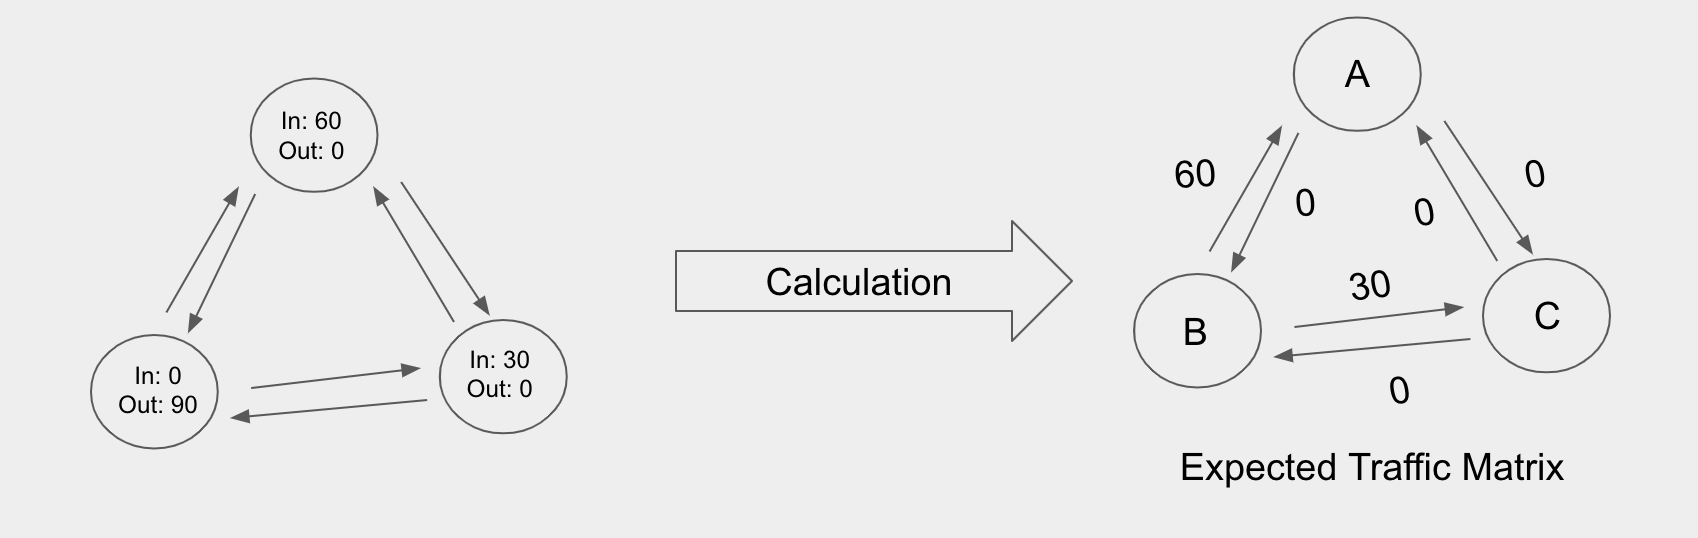
\includegraphics[width=10cm]{img/Simple_evaluation.png}
    \caption{Evaluation in Very Simple Case}
    \label{fig:eval_simple} 
\end{figure}
As shown in the figure, I use the case where the node data clearly shows the destination of all traffic.
You can see my actual test code from code listings \ref{eval_code}.
The test results correctly output the expected results, and the assertion test was passed.

For the unit test, I use Google Test to test the traffic matrix generation code that I have implemented.

\subsection{Traffic Matrix Generation Errors}
Next target is to verify that the generated traffic matrix is correct.
To evaluate the generated traffic matrix, various measures of errors are used.
The purpose of this is to compare the original traffic matrix and the generated traffic on an error scale to see how well the gravity model reproduces the characteristics of the original traffic.

The measures used in this project are Mean Squared Error (MSE), Root Mean Squared Error (RMSE), Mean Absolute Error (MAE), and Mean Absolute Percentage Error (MAPE).
As functions, I used library functions from scikit-learn.
See this page for definitions of measures of errors I used for this project.\cite{scikit-learn}

The following table transforms a randomly generated 12$\times$12 traffic matrix from a uniform distribution into node data. 
Based on the node data, the traffic matrix is generated by the function I implemented. 
This randomly generated traffic matrix from a uniform distribution is taken as the true value, and I evaluate how well my traffic matrix generator represents the original features using measures of errors.
\begin{table}[H]
    \centering
      \caption{Generation Errors}
      \label{table:loss}
      \small
      \begin{tabular}{|c||l|l|l|l|l|}  \hline
        Error & Mean & Median & Std & Min & Max \\ \hline
        MSE & 632.4389 & 630.6597 & 61.1020 & 461.3056 & 815.0278 \\
        RMSE & 24.7900 & 24.7868 & 1.2391 & 20.9479 & 28.3213 \\
        MAE & 20.2920 & 20.2639 & 1.2122 & 16.2083 & 23.8056 \\
        MAPE & 1.5686+e15 & 1.3448+e15 & 1.4074+e15 & 0.6073 & 9.3512+e15 \\ \hline
      \end{tabular}
\end{table}

The MAPE results are arbitrarily large. 
This is due to a feature of MAPE, which is that when the true value is close to zero, an extremely large value is output as the result.

In this project, there is no comparison to the gravity model. 
Therefore, it is important to note that this result does not imply that the gravity model is superior for generating quantum Internet traffic.
This will be the basis for the evaluation of traffic generation models for the Quantum Internet, which will increase in the future.
%%% Local Variables:
%%% mode: japanese-latex
%%% TeX-master: "./thesis"
%%% End:
